\documentclass[a4paper]{article}

\usepackage[english]{babel}
\usepackage[utf8]{inputenc}
\usepackage{amsmath}
\usepackage{graphicx}
\usepackage[colorinlistoftodos]{todonotes}

\title{%
  Proyecto final \\
  \\\\
  \large Sistemas Inteligentes (Grado en Ingeniería Informática) \\
    Universidad de La Laguna}

\author{Alberto Jesús González Álvarez, \\ Cristian Manuel Abrante Dorta}

\date{Enero, 2019}

\begin{document}
\maketitle

\section{Propuesta}
\subsection{Descripción}
La detección de objetos es un problema clásico en las disciplinas de visión por computador e
inteligencia artificial. De manera básica, consiste en reconocer que objetos están presentes en una determinada imagen. \\

El hecho de reconocer objetos en una imagen es una tarea cuya reproducción mediante ordenadores 
entraña enormes dificultades. Pero a la vez, un resultado satisfactorio puede tener muchas 
repercusiones en diversos ámbitos: implementación de robots o coches autónomos, mejora de las cámaras 
de seguridad, aumento de la precisión de los sensores biométricos, detección médica ... \\

El hecho de presentar tantas ventajas ha hecho que se haya convertido en una de las disciplinas 
centrales de la visión por computador. Sin embargo, ha tenido un desarrollo muy lento, limitado 
principalmente por la capacidad de cómputo de los ordenadores de la época y por las lentas mejoras en 
inteligencia artificial y aprendizaje automático.\\

De hecho, Las más importantes contribuciones a esta disciplina se han hecho en los últimos 20 
años. Desencadenadas principalemente por el aumento del poder de cómputo, la miniaturización de los 
componentes y la introducción de las técnicas de Deep Learning, surgidas a partir del año 2012. \\

Sin embargo, ha habido muchos intentos de algoritmos de inteligencia artificial encaminados hacia la detección de objetos, hasta llegar al punto actual de la disciplina:

\begin{itemize}
    \item \textbf{SIFT} (\textit{Scale Invariant Feature Transform}) (1999): Este algoritmo fue 
    desarrollado por D. G. Lowe en 1999, e incialmente fue utilizado para obtener las características 
    más relevantes de una imagen, las cuales posteriormente serían aplicadas al reconocimiento de 
    objetos y rostros.
    \item \textbf{Viola-Jones} (2001): Este algoritmo está principalmente motivado por el problema de 
    detección facial. Fue desarrollado por Paul Viola y Michael Jones en el año 2001, y hoy en día sigue siendo uno de los principales algoritmos en cuanto a reconocimiento facial, en parte gracias a su eficiente implementación en la famosa librería OpenCV. 
    \item \textbf{HOG} (\textit{Histogram Of Gradients}) (2005): La idea detrás de esta técnica es 
    utilizar el gradiente de la imágen en cada posición como posible característica invariante de los 
    objetos que se desean reconocer.
    \item \textbf{Deep Learning} (2012): La introducción de las técnicas de Deep Learning han sido cruciales en la mejora de la detección de objetos. Destaca especialmente la introducción de las 
    \textbf{Redes neuronales convolucionales} (CNN), las cuales son ampliamente utilizadas en esta 
    disciplina.
    \item \textbf{YOLO} (You Only Look Once) (2014): Esta técnica de reconocimiento de objetos se 
    considera el \textit{estado del arte} en el campo, y es la que trataremos de implementar.
\end{itemize}
\\
Tal y como hemos comentado, en este proyecto implementaremos el algoritmo \textbf{YOLO} (You Only Look
Once), en sus tres versiones diferentes. Este método basado en redes neuronales convolucionales fue 
desarrollado por Joseph Redmon y Anelia Angelova en el año 2015. Rápidamente adquirió una enorme 
relevancia debido principalemente a su eficiencia y buenos resultados. A partir de ahí surgieron tres 
versiones más de esta técnica, la última publicada en 2018.\\

La implementación original de este algoritmo se denomina Darknet, y está desarrollada en el lenguaje 
C, contando a su vez con aceleración mediante la GPU utilizando la API CUDA. Nuestra implementación no
se basará tanto en la eficiencia, sino en la usabilidad, puesto que realizaremos una aplicación web, la cual llevará a cabo \textbf{toda la carga computacional en el cliente}.\\

A su vez, desarrollaremos una interfaz gráfica que permitirá visualizar los resultados del algoritmo 
de una manera sencilla.

\subsection{Proyectos similares}
Los proyectos en los que nos hemos inspirado a la hora de llevar a cabo nuestra implementación han sido los siguientes:

\begin{figure}[ht]
    \centering
    
\includegraphics[scale=0.15]{images/darknet.png}
    \caption{Logo de Darknet}
    \label{fig:my_label}
\end{figure}
    
\begin{itemize}
    \item \textbf{Darknet} [4]: A raíz del desarrollo de YOLO, Joseph Redmon, trató de llevar a cabo 
    una implemtación real. El resultado de esto es Darknet, un framework de desarrollo de redes 
    neuronales en el lenguaje C y con aceleración de cálculo mediante la GPU, y la API CUDA. Para 
    nuestro proyecto es un buen punto de partida, sin embargo, esta implementación está hecha a muy 
    bajo nivel y utilizando APIs de acelaración que no están disponibles en un navegador.
    \item \textbf{Implementación de YOLO en PyTorch} [5]: En el campo del aprendizaje automático, el 
    lenguaje Python ha tomado una gran relevancia. De hecho, existen una gran diversidad de frameworks
    que se pueden utilizar, de entre los cuales uno de los más famosos es Pytorch. Este tutorial es
    muy interesante porque ofrece una visión paso a paso sobre la implementación de YOLO, utilizando 
    previamente la especificación de la red Darknet. Es muy iluistrativo a la hora de entener el 
    verdadero funcionamiento del procedimiento, sin embargo, no puede ser utilizado en la web, debido 
    a que el framework PyTorch no ofrece una versión para el navegador.
    \item \textbf{Implementación de YOLO usando Tensorflow.js} [6]: El autor de este proyecto 
    desarrolló una implementación de YOLO como aplicación web utilizando Tensorflow.js, lo cual es muy
    parecido a lo que realizamos en este proyecto. Sin embargo, la principal diferencia es que este 
    autor solo se limitó al reconocimiento de fotografías, y no realizó procesamiento de video.
\end{itemize}

\subsection{Recursos a usar}
Para la realización de este proyecto hemos utilizado principalmente estas tres tecnologías:

\subsubsection{React}

\begin{figure}[ht]
    \centering
    
\includegraphics[scale=0.05]{images/react-logo.png}
    \caption{Logo de React}
    \label{fig:my_label}
\end{figure}

Aunque no se trata de una herramienta relacionada con el \textit{Machine Learning}, ha sido el 
framework que hemos usado para construir nuestra aplicación web. React es una librería de código 
abierto desarrollada por Facebook y que permite llevar a cabo la implementación web con una 
aproximación orientada a componentes.\\

El lenguaje con el que trabaja es JavaScript, lo cual es muy útil puesto que podremos utilizar las 
librerias de deep learning disponibles para este lenguaje.

\subsubsection{Tensorflow.js}

\begin{figure}[h]
    \centering
    
\includegraphics[scale=0.3]{images/tfjs-logo.png}
    \caption{Logo de Tensorflow.js}
    \label{fig:my_label}
\end{figure}

Tensorflow.js es una extensión del framwork Tensorflow para el lenguaje JavaScript, el cual tiene 
originalmente APIs disponibles para los lenguajes Python y C++. Tensorflow fue desarrollado por Google
para llevar a cabo la implementación de funcionalidades de inteligenicia artificial en toda su 
\textit{suite} de aplicaciones. Tras esto, fue liberado como proyecto Open Source, ganando una enorme 
populariadad. \\

Con Tensorflow.js la intención es trasladar toda la potencia que ofrecía este framework a los 
navegadores,para ejecutar y entrenar modelos de aprendizaje automático en el lado del cliente.
En nuestra aplicación este framework será utilizado para cargar un modelo previamente entrenado y 
compilado en formato JSON, y poder ejecutarlo en el lado del cliente. \\

\subsubsection{Keras}

\begin{figure}[ht]
    \centering
    
\includegraphics[scale=0.1]{images/keras.png}
    \caption{Logo de keras}
    \label{fig:my_label}
\end{figure}

Keras es una librería para la especificación de modelos de redes neuronales en alto nivel. La gran 
ventaja de esta librería es que al especificar un modelo, este puede ser compilado para ser utilizado 
en diferentes frameworks como Tensorflow, Pytorch o Microsft Cognitive Toolkit. \\

En nuestro proyecto, hemos utilizado un modelo de Keras que posteriormente ha sido compilado a 
Tensorflow.js (Obteniendo un modelo en formato JSON).

\subsection{Tecnologías de IA utilizadas}
En este apartado explicaremos las dos principales herramientas o tecnologías de IA que pretendemos implementar.
\subsubsection{Redes neuronales convolucionales}
La creación de las redes neuronales convolucionales (CNN) representó un gran avance en el campo de la
visión por computador. Constituyen un mecanismo para procesar imágenes que trata de asemejarse a la
visión biológica, estableciendo una jerarquía que pasa de patrones visuales más explicítos a otros
más abstractos, a medida que se se utilizan capas más profundas en la red.

\begin{figure}[ht]
    \centering
    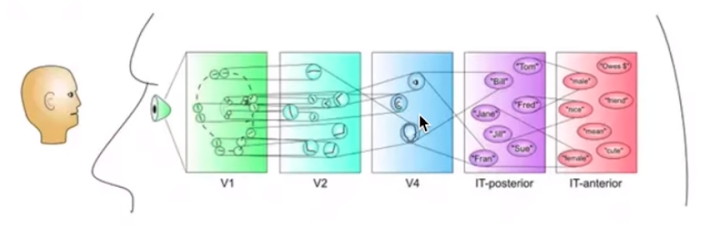
\includegraphics[scale=0.5]{images/cnn-1.png}
    \caption{Representación esquemática de una CNN}
    \label{fig:my_label}
\end{figure}

Estás redes neuronales constan de cuatro elementos principales:

\begin{figure}[ht]
    \centering
    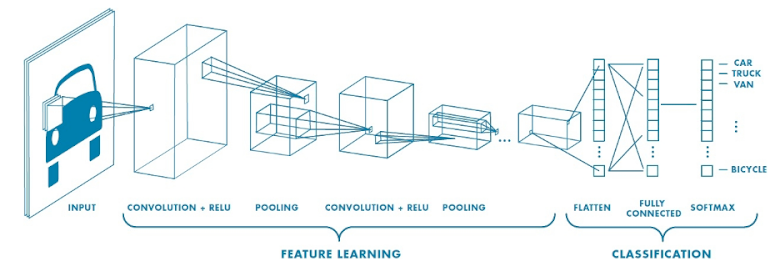
\includegraphics[scale=0.35]{images/cnn-2.png}
    \caption{Elementos principales de las CNN}
    \label{fig:my_label}
\end{figure}

\begin{itemize}
    \item \textbf{Convolución}: La convolución es una operación muy común en el procesamiento de 
    imágenes. Consiste en filtrar una imagen con un determinado \textit{kernel}, que
    no es más que una matriz bidimensional de pesos, en las cuales se realiza una multiplicación con
    los valores de pixeles presentes en la imagen. Esta técnica es muy útil a la hora de descubrir
    formas y patrones.
    \item \textbf{Pooling}: El procesamiento de una red neuronal convolucional es bastante complejo, 
    por lo que es necesario utilizar técnicas que reduzcan la complejidad de este problema. Una de 
    estas técnicas es el \textit{Pooling}, la cual se utiliza para reducir el tamaño de las imágenes
    intermedias. Hay diversos tipos de \textit{Pooling}, por ejemplo, el \textit{Max-pooling}, que 
    trata de reducir una vecindad de pixeles a uno solo, buscando el máximo en dicha vecindad.
    \item \textbf{Relu}: Esta técnica trata de normalizar los pesos obtenidos tras los pasos de 
    convolución y pooling, de tal forma que no existan pesos negativos.
    \item \textbf{Clasificación}: En la tarea de clasificación, es necesario asignar un valor de 
    probabilidad a cada una de las clases que se estén tratando. Para ello, se aplica
    la función exponencial normalizada (\textit{SoftMax}), a la salida de la última capa de la red
    neuronal.
    \[\sigma : \mathbb{R}^{K} \rightarrow [0, 1]^K\]
    \[\sigma(z)_j = \frac{e^{zj}}{\sum^{K}_{k = 1}e^{zk}}\]
\end{itemize}

\subsubsection{YOLO (You Only Look Once)}
Yolo presenta un enfoque diferente a otros procedimientos existentes de reconocimiento de imágenes. 
Se basa en redes neuronales convolucionales, introduciendo algunas carácterísticas que producen
una mejora significativa en la eficiencia. \\

La red neuronal convolucional que utiliza Yolo posee 75 capas de convolución. El tamaño de entrada
de esta red son imágenes redimensionadas a 416 píxeles por 416 píxeles, para poder utilizar el 
procesamiento en \textit{batches}, es decir en lotes distribuidos en la GPU. \\

\begin{figure}[ht]
    \centering
    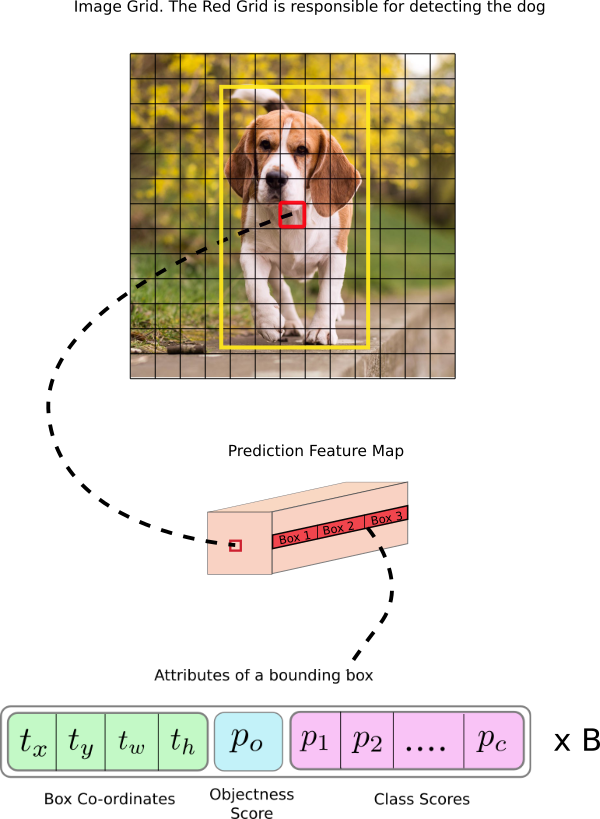
\includegraphics[scale=0.3]{images/yolo-1.png}
    \caption{Esquema que representa el resultado obtenido por cada una de las regiones}
    \label{fig:my_label}
\end{figure}

El funcionamiento de este procedimiento es el siguiente:

\begin{itemize}
    \item \textbf{División de la imagen en regiones}: La imagen se divide en regiones de 13 píxeles 
    por 13 píxeles. Estas regiones servirán para predecir tanto los \textit{bounding boxes} (regiones
    donde se encuentran los objetos), como la clase de dicho objeto. Cabe destacar que cada región 
    solo podrá predecir hasta 5 \textit{bounding boxes} diferentes.
    \item \textbf{Se ejecuta el modelo sobre la imagen}: Al ejecutar el modelo sobre la imagen 
    obtendremos un vector (o un \textit{Tensor} en la terminología de Tensorflow), que contiene un 
    conjunto de elementos: la posición de la esquina superior izquierda del \textit{bounding box} (x e
    y), el alto y ancho del \textit{bounding box}, el nivel de confianza de la predicción y finalmente
    una probabilidad por cada una de las clases que se estén clasificando. Todo este tamaño se
    multiplica por 5, es decir, el número de \textit{bounding boxes}
    por cada región.
    \item \textbf{Procesamiento del vector de resultados}: Una vez obtenido este vector se procesa,
    obteniendo la clase con mayor probabilidad y descartando aquellas que tengan un nievel de 
    confianza inferior a un determinado umbral, en nuestro caso, del 30\%.
\end{itemize}

Cabe destacar que desde su desarrollo, se han creado 3 versiones del procedimiento diferentes 
(\textit{v1}, \textit{v2}, \textit{v3}) y unas versiones simplificadas, denominadas
\textit{Tiny}. Las mejoras introducidas en cada versión suelen incidir en la eficiencia,
introudciendo alguna característica significativa como el uso de \textit{anchors} o proporciones 
predefinidas para calcular la menor cantidad de \textit{bounding boxes} posibles.

\section{Desarrollo}
\subsection{Lista de tareas y cronograma}
El cronograma seguido durante el desarrollo del proyecto ha sido el siguiente:

\begin{figure}[ht]
    \noindent\makebox[\textwidth]{%
    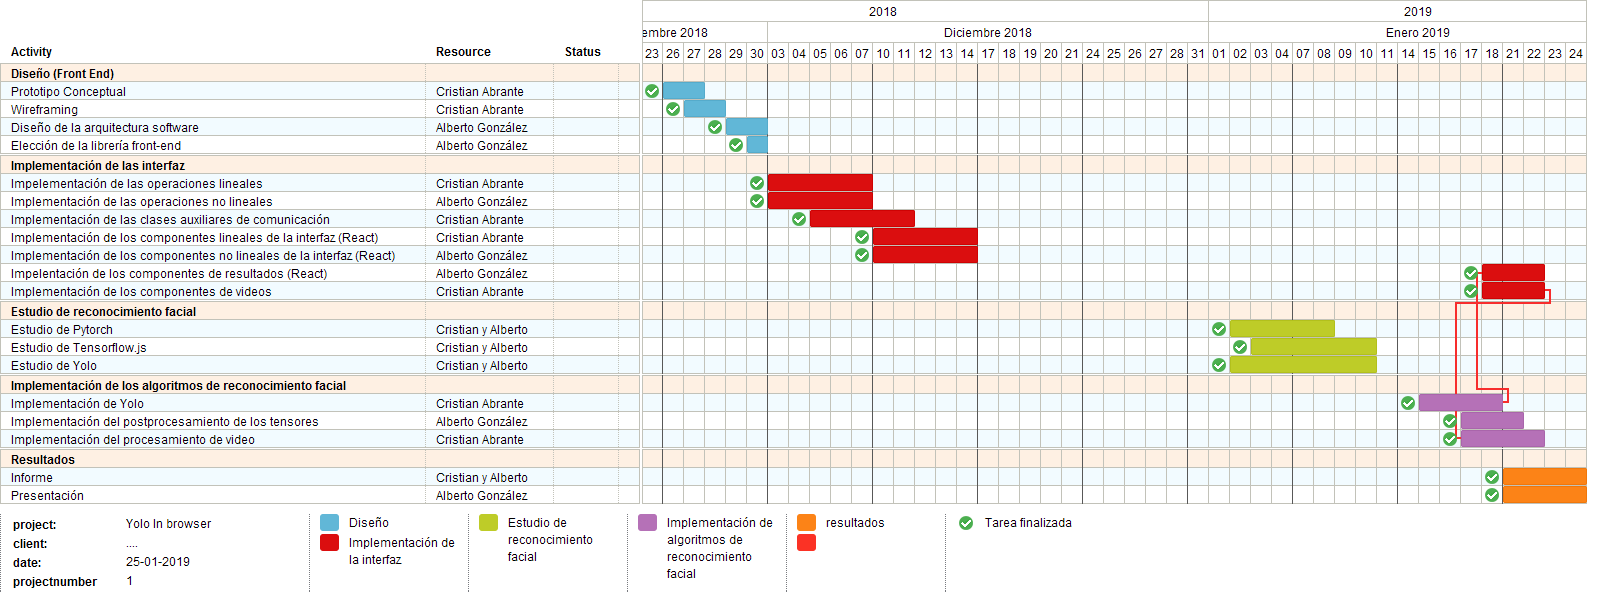
\includegraphics[scale=0.4]{images/SI.png}}
   \caption{Cronograma del proyecto}
\end{figure}

Este cronograma puede dividirse en 4 grandes grupos de tareas:

\begin{itemize}
    \item \textbf{Diseño (front end)}: Estas tareas se corresponden al diseño preliminar de la 
    aplicación. En ellas hemos realizado tanto el diseño visual como el diseño lógico. Es una fase 
    relativamente sencilla, puesto que ya habíamos trabajado previamente con la librería React, lo
    que simplificó el desarrollo.
    \item \textbf{Impelementación de la interfaz}: Para implementar la interfaz utilizamos la librería
    React,un desarrollo que se extendió alrededor de dos semanas, y en el cual implementamos no solo 
    la parte visual,sino también las principales herramientas que nos permiten trabajar con imágenes: 
    operaciones lineales y no lineales. Finalmente, una vez que los algoritmos ya estuvieron 
    implementados, desarollamos las clases que permitian mostrar los resultados.
    \item \textbf{Estudio de loa algoritmos de reconocimiento de objetos}: No solo estudiamos el 
    algoritmo YOLO, sino que también fue necesario estudiar los principales frameworks de desarollo de
    aprendizaje automático.
    \item \textbf{Implementación de algoritmos de reconocimiento de objetos}: Esta fase se 
    corresponde con la implementación de YOLO, tanto para el reconocimiento de objetos en fotografías 
    como en videos. Además, fue necesario llevar a cabo un procesamiento de la información devuelta
    por el algoritmo.
    \item \textbf{Resultados}: Esta es la fase final del proyecto, se corresponde con la elaboración del informe y la presentación de los resultados.
\end{itemize}

\subsection{Problemas encontrados}
Durante el desarrollo de este proyecto nos hemos encontrado con una serie de problemas que hemos 
tenido que ir solventando. El primero de todos, ha sido el proceso de estudio de los diferentes 
frameworks de aprendizaje automático. Estas librerías ofrecen APIs extensas que para ser entendidas 
con profundidad requieren de meses de trabajo, sin embargo nosotros no disponemos de ese tiempo. \\

El segundo gran problema que hemos encontrado ha sido la dificultad que tienen aparejadas las 
aplicaciones web que requieren de abundantes recursos computacionales para funcionar. Creemos que fue 
una decisión bastante arriesgada el llevar a cabo una aplicación que realice toda la carga 
computacional en el lado del cliente (y por tanto en el navegador), más aun teniendo en cuenta que 
este algoritmo requiere de aceleración de GPU para funcionar correctamente. \\

Esta dificultad se ha visto incrementada sobretodo cuando tratamos de procesar video a tiempo real. Al
no contar con la potencia de cálculo que ofrece una GPU dedicada, y ni siquiera poder ejecutar el 
modelo de manera nativa, el tiempo de procesamiento se ve aumentado enormemente, llegando a perder la 
capacidad de realizar el procesamiento en tiempo real.\\

Sin embargo, esta pérdida de rendimiento se ve aparejada por una enorme mejora en flexibilidad. Pues 
esta aplicación puede ser ejecutada en navegadores de dispositivos móviles, ofreciendo una aplicación 
completa de procesamiento de imágenes y reconocimiento de objetos de manera sencilla en nuestros smartphones.\\

Finalmente, otra de las dificultades encontradas se corresponde con las diferencias que tienen las 
aplicaciones web a la hora de ejecutarse en navegadores diferentes. De esta forma, nuestra aplicación 
puede obtener resultados de procesamiento distintos dependiento del navegador donde sea ejecutado.

\subsection{Requisitos y objetivos alcanzados}
Los requisitos y objetivos alcanzados pueden dividirse en requisitos de procesamiento de imágenes y de video.

\begin{itemize}
    \item \textbf{Procesamiento de imágenes}: En cuanto al procesamiento de imágenes individuales se 
    han logrado resultados muy satisfactorios. Por una parte, se ha logrado procesar imágenes de 
    tamaños diversos, tanto subidas por el usuario como imágenes de muestra. Por otra parte, la 
    interfaz en la que se muestran los resultados es bastante ilustrativa, de tal forma que el usuario
    puede observar cual ha sido el resultado del algoritmo de una manera muy visual.
    \item \textbf{Procesamiento de video}:  El procesamiento de video a tiempo real es una tarea 
    demasiado compleja como para llevarla a cabo satisfactoriamente con la potencia de cómputo que nos
    ofrece un navegador. Sin embargo, si que hemos podido llevar a cabo el procesamiento de un video, a través de una etapa de preprocesado, es decir, utilizando un \textit{buffer} en el que ir 
    calculando los objetos de la escena de antemano. Sin embargo, no hemos podido utilizar cualquier 
    video subido por el usuario, puesto que el video elegido ha sido previamente transformado de 
    formato y escalado para satisfacer las restricciones de entrada de yolo, ahorrando así tiempo de 
    procesamiento.
\end{itemize}

\section{Descripción del funcionamiento}
La aplicación que hemos desarrollado se denomina \textbf{YOLO in browser},  cuyo código puede ser 
consultado en \url{https://github.com/CristianAbrante/YOLO-in-browser}. Además, al tratarse de una 
aplicación web, pudimos desplegarla utilizando como \textit{host} el propio repositorio. Su 
dirección web es la siguiente:

\begin{center}
    \textbf{\url{https://cristianabrante.github.io/YOLO-in-browser/}} \\
\end{center}

Para describir el funcionamiento de la aplicación, analizaremos las dos principales funcionalidades
que presenta: el reconocimiento de objetos en imágenes, y el reconocimiento de objetos en video. \\

\subsection{Carga y selección del modelo}
Pero antes de hacer ningún procesamiento, debemos cargar el modelo en nuestra aplicación. Tal y como 
describimos anteriormente, nuestra aplicación permitirá 
utilizar la versión de yolo \textit{v1 tiny}, \textit{v2 tiny}, \textit{v3 tiny} o \textit{v3}. Esta
selección se hará a través de un cuadro de diálogo como el siguiente: \\

\begin{figure}[ht]
    \centering
    
\includegraphics[scale=0.4]{images/model-loader.png}
    \caption{Cuadro de diálogo para la carga del modelo}
    \label{fig:my_label}
\end{figure}

En este cuadro de diálogo, el usuario podrá seleccionar, mediante un menú deplegable, que versión de 
yolo es la que desea ejecutar, pudiendo elegir la opción de cargar la versión \textit{tiny}. \\

Cuando se presione el botón \textit{Load Model} se comenzará a descargar el fichero
JSON que contiene el modelo, y que está alojado en el repositorio indicando mediante un \textit{spinner} el progreso de la descarga. \\

\begin{figure}[ht]
    \centering
    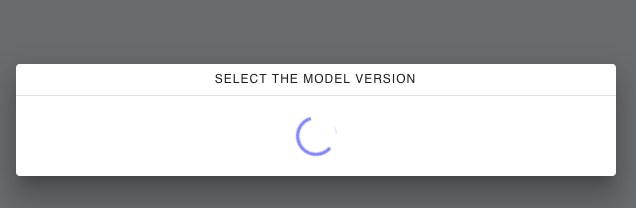
\includegraphics[scale=0.4]{images/model-loading.png}
    \caption{Progreso de la descarga del modelo}
    \label{fig:my_label}
\end{figure}

Una vez el modelo se ha cargado correctamente, se cerrará este cuadro de diálogo, pudiendo ser 
utilizado durante todo lo que dure la sesión sin tenerlo que recargar nuevamente.

\subsection{Reconocimiento de objetos en imágenes}
Para llevar a cabo el reconocimiento de los objetos presentes en una imagen, en primer lugar debemos
seleccionar la imagen que qeremos procesar: \\

\begin{figure}[ht]
    \centering
    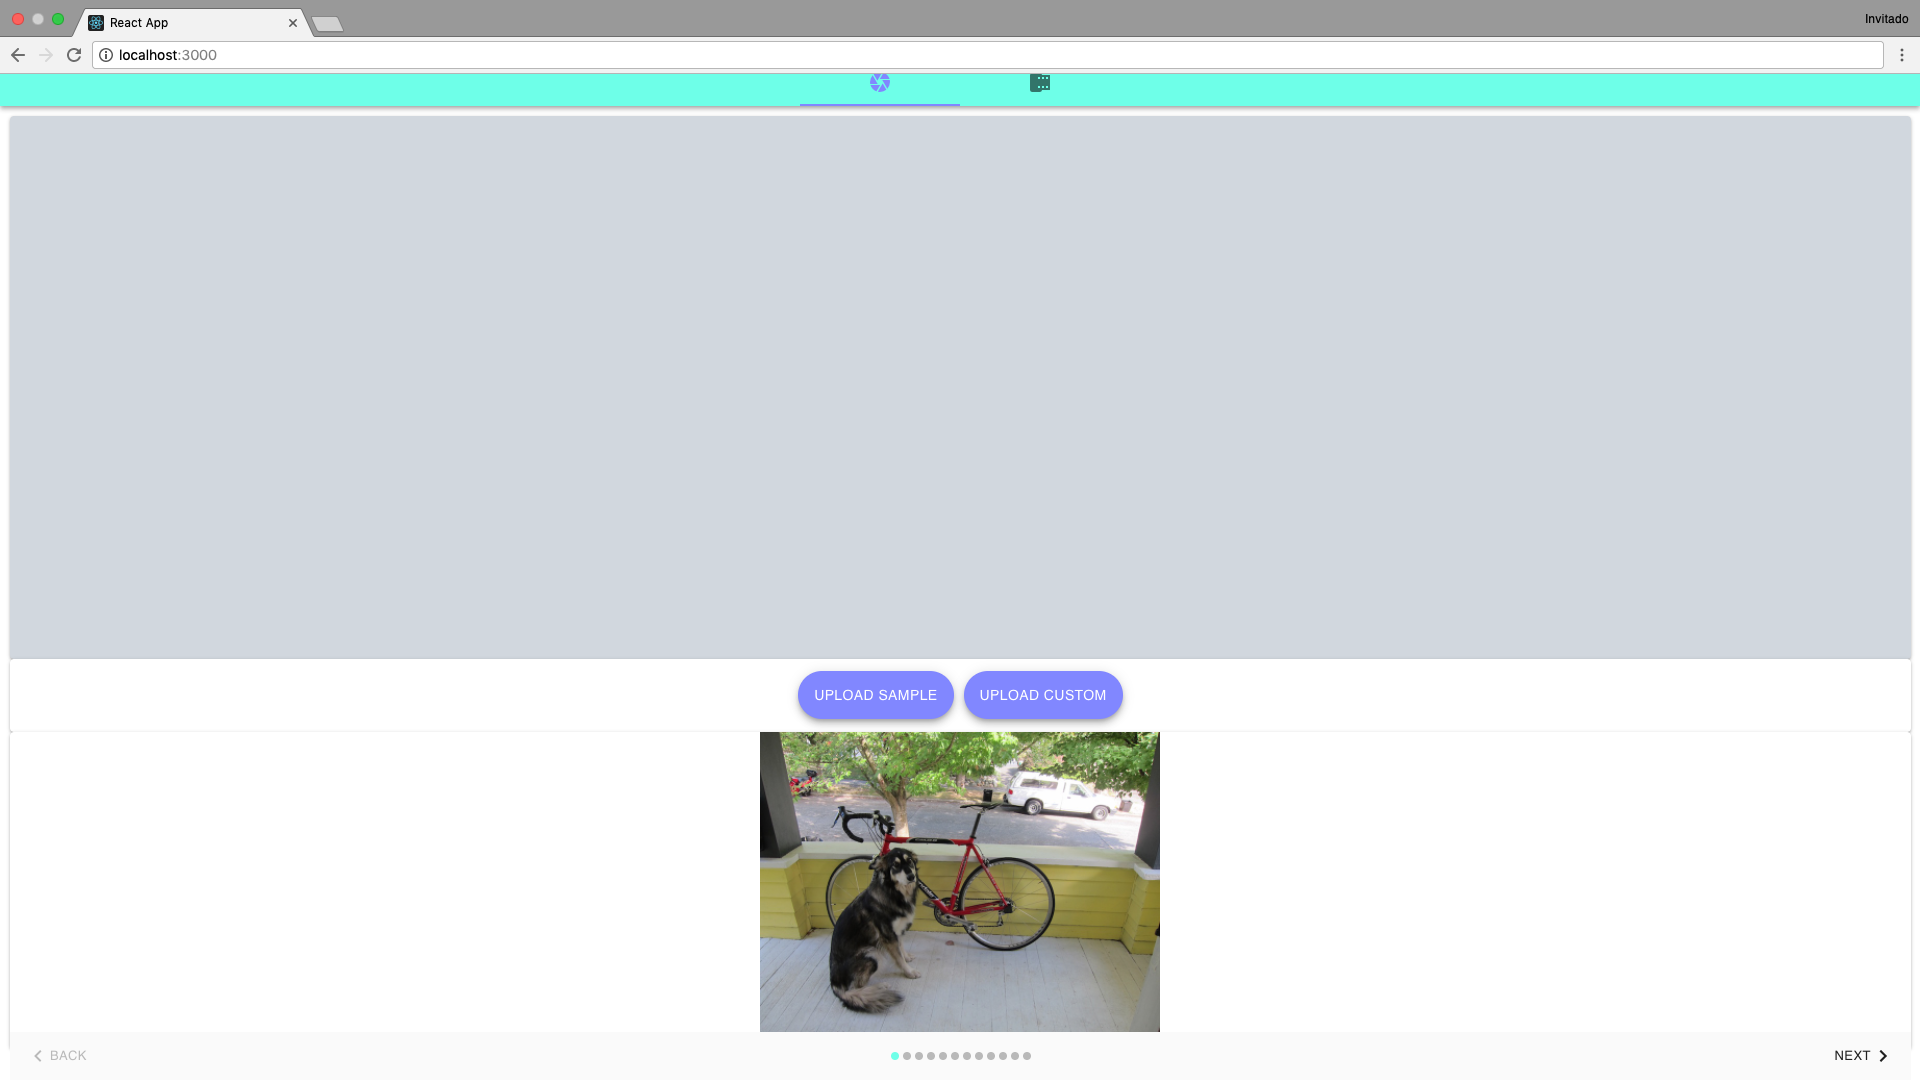
\includegraphics[scale=0.15]{images/image-selection.png}
    \caption{Interfaz principal de selección de imágenes}
    \label{fig:my_label}
\end{figure}

En esta interfaz podremos elegir la imagen que queremos que sea procesada. Pudiendo seleccionar entre 
una galería de ejemplos clásicos de procesamiento de imágenes o cargar nuestra propia imagen desde el 
sistema de archivos. Esta selección se realizará pulsando uno de los botones presentes en la 
interfaz.\\

Una vez que se ha cargado la imagen se procesará con el modelo previamente cargado, y se mostrará 
inmediatamente la pantalla de resultado:

\begin{figure}[ht]
    \centering
    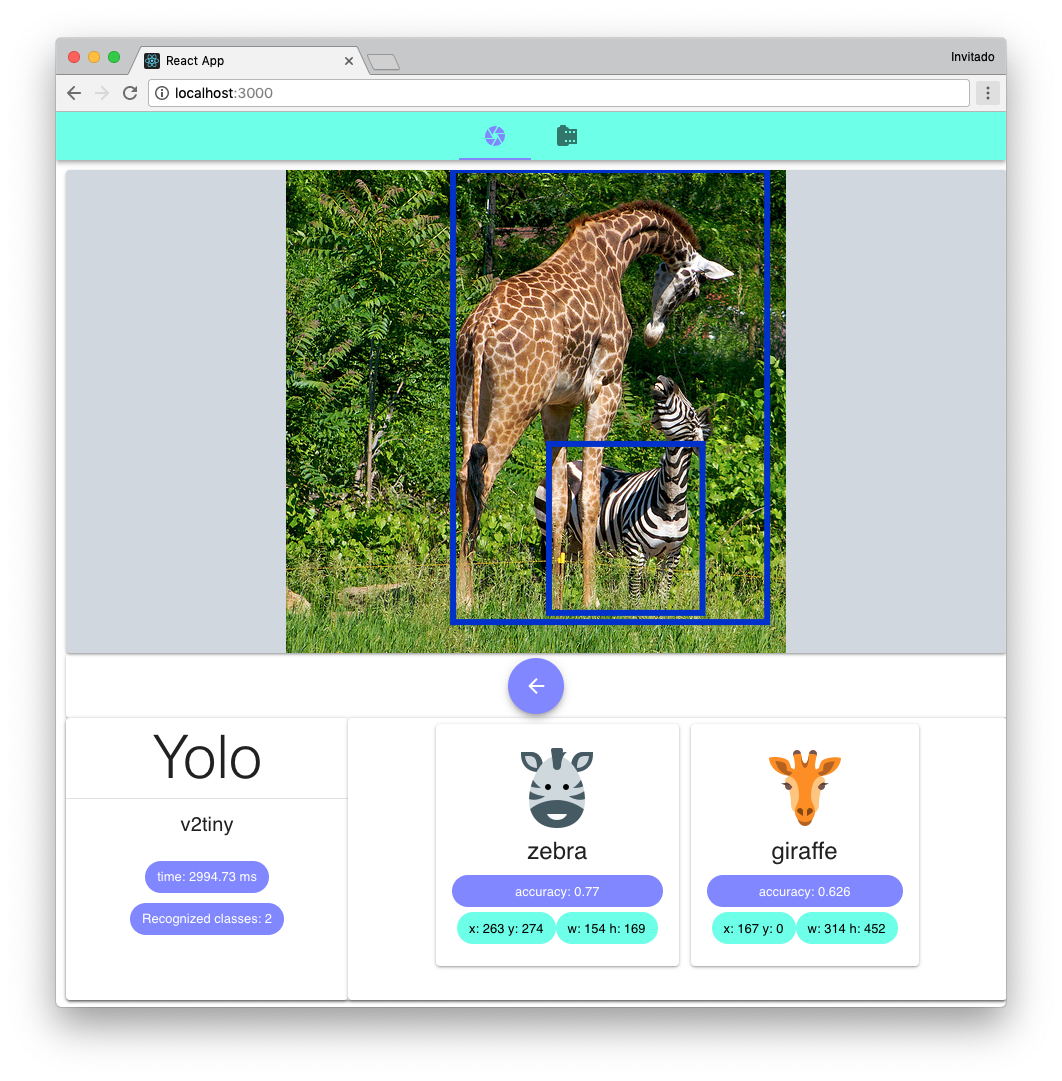
\includegraphics[scale=0.3]{images/result-1.png}
    \caption{Resultado mostrado con una imagen a procesar}
    \label{fig:my_label}
\end{figure}

Esta pantalla de resultados muestra diferente información. Por una parte, imprime la imagen escalada a
un mayor tamaño, señalando los \textit{bounding-boxes} donde se inscriben los objetos que se han podido reconocer. \\ 

Además de esto, dicha pantalla pone de manifiesto el desempeño del algoritmo. Mostrando por una parte,
el tiempo que ha tardado en realizar el procesamiento, y el número total de clases que ha logrado 
reconocer.  \\

Además, la información de cada una de las clases reconocidas se extiende en la pantalla
contigua, mostrando cada una de ellas en un recuadro, en el que tambén se indica la
probabilidad o confianza con la que esta clase es reconocida. Mostrando a su vez las características 
del \textit{bounding box}, como son la posición bidimensional de la esquina superior izquierda (en 
coordenadas de píxeles x e y) y el ancho y alto de dicho recuadro.

\subsection{Reconocimiento de objetos en video}
En cuanto al reconocimiento de objetos en video, cabe destacar que no se realizará en tiempo real,
debido a las limitaciones que presenta la computación web, especialmente la realizada en el lado 
del cliente. Es por ello, que al elegir esta opción nos saldrá la siguiente ventana:

\begin{figure}[ht]
    \centering
    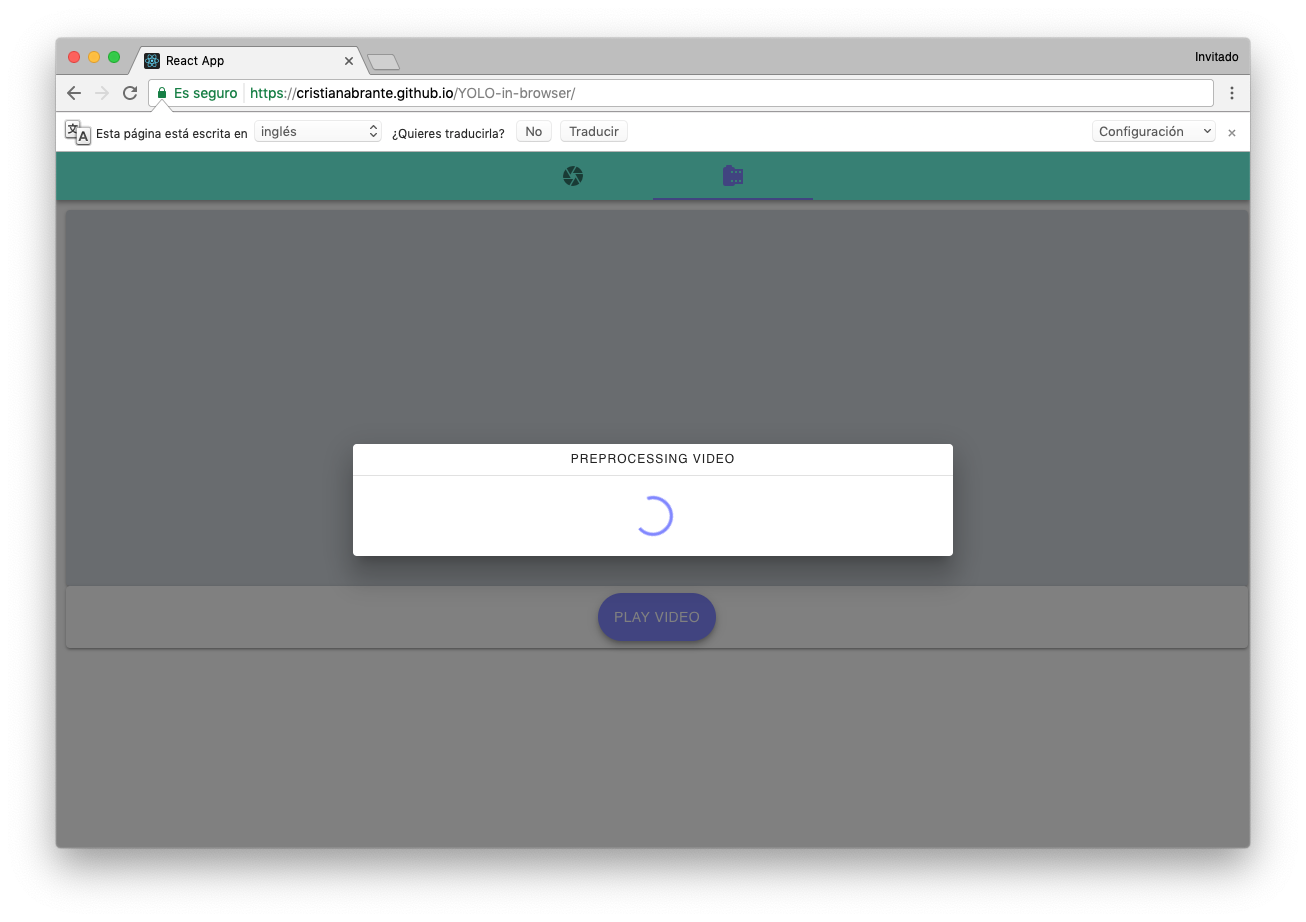
\includegraphics[scale=0.25]{images/video-loading.png}
    \caption{Pantalla que indica el preprocesamiento del video}
    \label{fig:my_label}
\end{figure}

Esta ventana indica que al video que hemos elegido como ejemplo de funcionamiento se le está aplicando
un preprocesamiento que consta de varias fases. \\

en primer lugar, el video es escalado a un tamaño de 416 píxeles de ancho por 416 píxeles de alto, es 
decir, a la entrada de la red neuronal de Yolo. Esto se hace para evitar consumir tiempo de 
procesamiento en escalar el \textit{canvas} en el que se están procesando los frames del video. \\

La segunda fase consiste en elegir un \textit{buffer} de frames para que se vaya procesando de 
antemano. Eligiendo un \textit{frame rate}, o número de frames que se procesarán, adecuado se puede
consegir un resultado que se pueda procesar en un tiempo razonable. En nuestro caso, este 
\textit{frame rate} es de 200 milisegundos. Es decir, que cada 200 milisegundos se llamará a la 
función de procesado de la imagen. \\

Finalmente, cabe destacar que una vez el video se haya procesado, este será almacenado temporalmente
en la sesión, es decir que se podría reproducir de nuevo sin tener que recalcularlo.

\section{Conclusiones y lineas futuras}

En general, consideramos que el resultado de este proyecto ha sido bastante satisfactorio, sobretodo
porque hemos conseguido implementar una aplicación de reconocimiento de objetos, lo cual es 
computacionalmente muy costoso, en el navegador. Al no existir demasiados antecedentes en este 
ámbito, sobretodo debido al poco tiempo que llevan en el mercado los frameworks como Tensorflow.js,
creemos que se ha hecho un tabajo más que aceptable, teniendo en cuenta las limitaciones físicas
de los dispositivos a los que va dirigida. \\

Como lineas futuras de desarrollo, destacamos la mejora del procesamiento de video, intentando 
llevarlo a cabo sin tener que hacer un cambio de escala en el mismo y mejorando la velocidad de 
cómputo de cada uno de los frames. Esto hoy en día es complejo, puesto que aun no se ha implementado 
de manera nativa para los navegadores los procedimientos de aceleración de cálculo que si están 
presentes en otras plataformas.

\begin{thebibliography}{9}
\bibitem{DGLowe}
    D. G. Lowe
    \newblock {\em Object recognition from local scale-invariant features}.
    \newblock {\em Proceedings of the Seventh IEEE International Conference on Computer Vision}, 1999.
    
\bibitem{ViolaJones}
    P. Viola and M. Jones
    \newblock {\em Robust real-time face detection}.
    \newblock {\em Proceedings Eighth IEEE International Conference on Computer Vision}, 2001.
    
\bibitem{yolo}
    Joseph Redmon and Anelia Angelova
    \newblock {\em Real-Time Grasp Detection Using Convolutional Neural Networks}.
    \newblock {\em Proceedings Eighth IEEE International Conference on Computer Vision}, 2015.
    
\bibitem{yolo}
    Joseph Redmon
    \newblock {\em Darknet: Open Source Neural Networks in C}.
    \newblock {\em \url{http://pjreddie.com/darknet/}}, 2013 - 2016.
    
\bibitem{yolo}
    Ayoosh Kathuria
    \newblock {\em How to implement a YOLO (v3) object detector from scratch in PyTorch}.
    \newblock {\em \url{https://blog.paperspace.com/how-to-implement-a-yolo-object-detector-in-pytorch/}}, 2018.
    
\bibitem{yolo}
    Piotr Skalski
    \newblock {\em In-Browser object detection using YOLO and TensorFlow.js}.
    \newblock {\em \url{https://towardsdatascience.com/in-browser-object-detection-using-yolo-and-tensorflow-js-d2a2b7429f7c}}, 2018.

\end{thebibliography}

\end{document}